\documentclass{article}\usepackage{graphicx, color}
%% maxwidth is the original width if it is less than linewidth
%% otherwise use linewidth (to make sure the graphics do not exceed the margin)
\makeatletter
\def\maxwidth{ %
  \ifdim\Gin@nat@width>\linewidth
    \linewidth
  \else
    \Gin@nat@width
  \fi
}
\makeatother

\IfFileExists{upquote.sty}{\usepackage{upquote}}{}
\definecolor{fgcolor}{rgb}{0.2, 0.2, 0.2}
\newcommand{\hlnumber}[1]{\textcolor[rgb]{0,0,0}{#1}}%
\newcommand{\hlfunctioncall}[1]{\textcolor[rgb]{0.501960784313725,0,0.329411764705882}{\textbf{#1}}}%
\newcommand{\hlstring}[1]{\textcolor[rgb]{0.6,0.6,1}{#1}}%
\newcommand{\hlkeyword}[1]{\textcolor[rgb]{0,0,0}{\textbf{#1}}}%
\newcommand{\hlargument}[1]{\textcolor[rgb]{0.690196078431373,0.250980392156863,0.0196078431372549}{#1}}%
\newcommand{\hlcomment}[1]{\textcolor[rgb]{0.180392156862745,0.6,0.341176470588235}{#1}}%
\newcommand{\hlroxygencomment}[1]{\textcolor[rgb]{0.43921568627451,0.47843137254902,0.701960784313725}{#1}}%
\newcommand{\hlformalargs}[1]{\textcolor[rgb]{0.690196078431373,0.250980392156863,0.0196078431372549}{#1}}%
\newcommand{\hleqformalargs}[1]{\textcolor[rgb]{0.690196078431373,0.250980392156863,0.0196078431372549}{#1}}%
\newcommand{\hlassignement}[1]{\textcolor[rgb]{0,0,0}{\textbf{#1}}}%
\newcommand{\hlpackage}[1]{\textcolor[rgb]{0.588235294117647,0.709803921568627,0.145098039215686}{#1}}%
\newcommand{\hlslot}[1]{\textit{#1}}%
\newcommand{\hlsymbol}[1]{\textcolor[rgb]{0,0,0}{#1}}%
\newcommand{\hlprompt}[1]{\textcolor[rgb]{0.2,0.2,0.2}{#1}}%

\usepackage{framed}
\makeatletter
\newenvironment{kframe}{%
 \def\at@end@of@kframe{}%
 \ifinner\ifhmode%
  \def\at@end@of@kframe{\end{minipage}}%
  \begin{minipage}{\columnwidth}%
 \fi\fi%
 \def\FrameCommand##1{\hskip\@totalleftmargin \hskip-\fboxsep
 \colorbox{shadecolor}{##1}\hskip-\fboxsep
     % There is no \\@totalrightmargin, so:
     \hskip-\linewidth \hskip-\@totalleftmargin \hskip\columnwidth}%
 \MakeFramed {\advance\hsize-\width
   \@totalleftmargin\z@ \linewidth\hsize
   \@setminipage}}%
 {\par\unskip\endMakeFramed%
 \at@end@of@kframe}
\makeatother

\definecolor{shadecolor}{rgb}{.97, .97, .97}
\definecolor{messagecolor}{rgb}{0, 0, 0}
\definecolor{warningcolor}{rgb}{1, 0, 1}
\definecolor{errorcolor}{rgb}{1, 0, 0}
\newenvironment{knitrout}{}{} % an empty environment to be redefined in TeX

\usepackage{alltt}
\usepackage[sc]{mathpazo}
\usepackage{geometry}
\geometry{verbose,tmargin=2.5cm,bmargin=2.5cm,lmargin=2.5cm,rmargin=2.5cm}
\setcounter{secnumdepth}{2}
\setcounter{tocdepth}{2}
\usepackage{url}
\usepackage[unicode=true,pdfusetitle, bookmarks=true,bookmarksnumbered=true,bookmarksopen=true,bookmarksopenlevel=2, breaklinks=false,pdfborder={0 0 1},backref=false,colorlinks=false] {hyperref}
\hypersetup{ pdfstartview={XYZ null null 1}}
\usepackage{breakurl}
\parindent = 0pt
\usepackage{amsfonts}
\usepackage{amsmath}
\usepackage{framed, color}
\definecolor{shadecolor}{RGB}{211, 211, 211}

\def\be{\begin{enumerate}}
\def\ee{\end{enumerate}}
\def\vh{\vskip0mm\hskip9mm}
\def\vn{\vskip0mm}
\def\vvn{\vskip0mm\noindent}
\def\vnn{\vskip0mm\noindent}
\def\h{\hskip4mm}
\def\bul{$\bullet$}
\def\P{\mathrm{Pr}}
\begin{document}



\begin{center}
{\bf MIKE LEDERLE - STATISTICS 641 - ASSIGNMENT 5}
\end{center}
\vskip0mm\noindent
\normalsize
\vnn\vnn
$\bullet$ Read Handouts 8 \& 9
\vnn\vnn
{\bf I.\ (6 points)}\ \   Suppose 50  iid
  observations $Y_1,Y_2,\ldots,Y_{50}$ from a process yield the following normal
  probability plot.

%   \begin{center}
%   \noindent
% \rotatebox{270}{
% \psfig{file=u:/exams/stat641/e1f06_Q1.ps,height=5in,width=3in}}
% \end{center}

Using the above plot, describe the shape of the process distribution.
\vskip3mm
\vvn
\begin{shaded}
{\bf I DON'T HAVE THE FIGS, SO I COULDN"T GENERATE THE GRAPHS}\\[5pt]
Looks like heavy-tails compared to a normal, like a $t$ with low df.
\end{shaded}
{\bf II.\ (15 points )}\ \  A researcher is studying the relative brain weights (brain weight divided by body weight) for 51 species of mammal whose average litter size is less than 2 and for 45 species of mamma whose average litter size is greater than or equal to 2. The researcher was interested in determining what evidence that brain sizes tend to be different for
    the two groups. (Data from {\it The Statistical Sleuth} by Fred Ramsey and Daniel Schafer).
  \vvn
  \footnotesize
  \begin{verbatim}
                   RELATIVE BRAIN WEIGHTS - SMALL LITTER SIZE

   0.42    0.86    0.88    1.11    1.34    1.38    1.42    1.47    1.63
   1.73    2.17    2.42    2.48    2.74    2.74    2.79    2.90    3.12
   3.18    3.27    3.30    3.61    3.63    4.13    4.40    5.00    5.20
   5.59    7.04    7.15    7.25    7.75    8.00    8.84    9.30    9.68
   10.32   10.41   10.48   11.29   12.30   12.53   12.69   14.14   14.15
   14.27   14.56   15.84   18.55   19.73   20.00

                   RELATIVE BRAIN WEIGHTS - LARGE LITTER SIZE

    0.94    1.26    1.44    1.49    1.63    1.80    2.00    2.00    2.56
    2.58    3.24    3.39    3.53    3.77    4.36    4.41    4.60    4.67
    5.39    6.25    7.02    7.89    7.97    8.00    8.28    8.83    8.91
    8.96    9.92   11.36   12.15   14.40   16.00   18.61   18.75   19.05
   21.00   21.41   23.27   24.71   25.00   28.75   30.23   35.45   36.35
  \end{verbatim}
  \normalsize
\vvn
\begin{enumerate}
\item[1.] Produce a q-q plot of the two data sets.
\begin{shaded}
\begin{knitrout}
\definecolor{shadecolor}{rgb}{0.969, 0.969, 0.969}\color{fgcolor}\begin{kframe}
\begin{alltt}
small <- \hlfunctioncall{c}(0.42, 0.86, 0.88, 1.11, 1.34, 1.38, 1.42, 1.47, 1.63, 1.73, 2.17, 2.42, 2.48, 2.74, 
    2.74, 2.79, 2.9, 3.12, 3.18, 3.27, 3.3, 3.61, 3.63, 4.13, 4.4, 5, 5.2, 5.59, 7.04, 7.15, 
    7.25, 7.75, 8, 8.84, 9.3, 9.68, 10.32, 10.41, 10.48, 11.29, 12.3, 12.53, 12.69, 14.14, 
    14.15, 14.27, 14.56, 15.84, 18.55, 19.73, 20)

large <- \hlfunctioncall{c}(0.94, 1.26, 1.44, 1.49, 1.63, 1.8, 2, 2, 2.56, 2.58, 3.24, 3.39, 3.53, 3.77, 4.36, 
    4.41, 4.6, 4.67, 5.39, 6.25, 7.02, 7.89, 7.97, 8, 8.28, 8.83, 8.91, 8.96, 9.92, 11.36, 
    12.15, 14.4, 16, 18.61, 18.75, 19.05, 21, 21.41, 23.27, 24.71, 25, 28.75, 30.23, 35.45, 
    36.35)

\hlfunctioncall{qqplot}(small, large)
\end{alltt}
\end{kframe}

{\centering 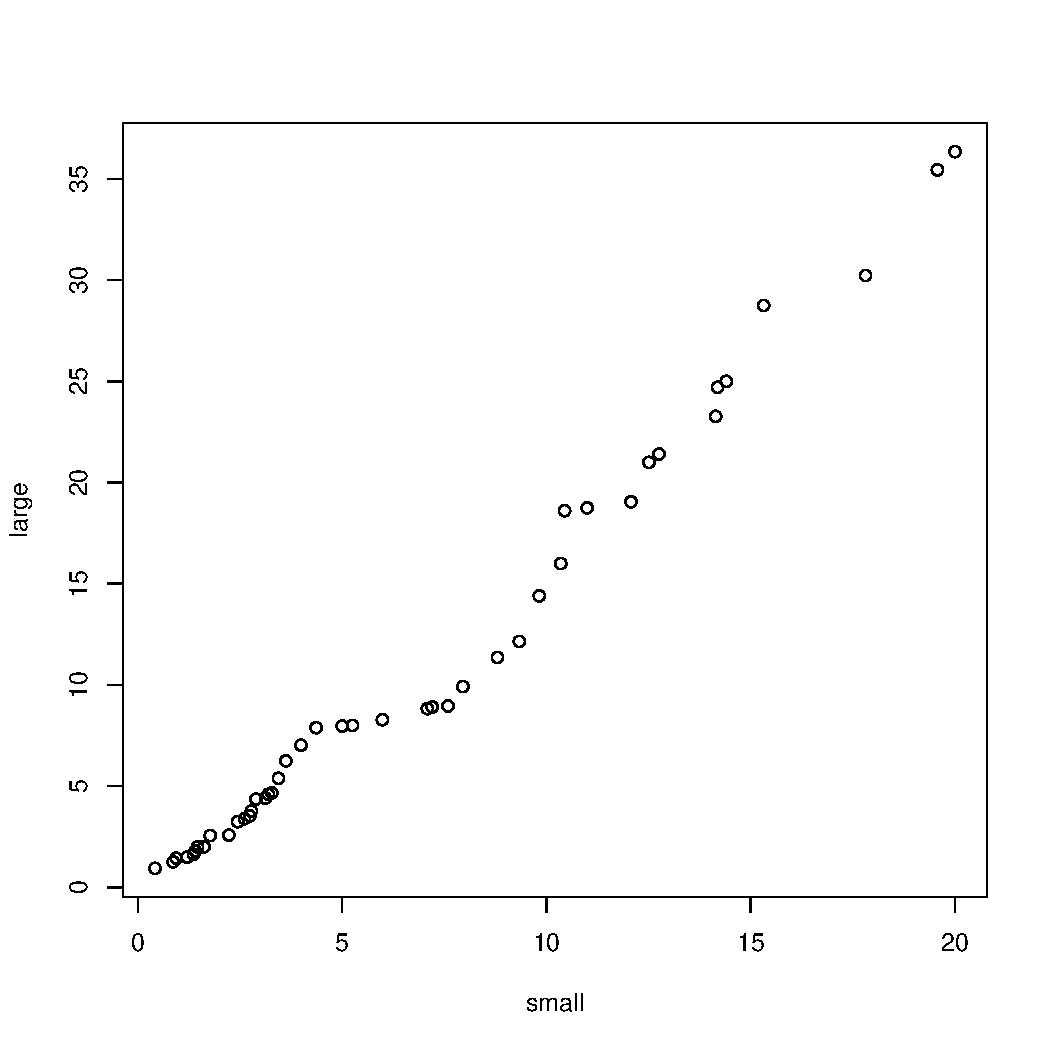
\includegraphics[width=.65\textwidth]{figure/unnamed-chunk-1} 

}


\end{knitrout}


\end{shaded}
\item[2.] Produce separate normal reference distribution plot.
\begin{shaded}
\begin{knitrout}
\definecolor{shadecolor}{rgb}{0.969, 0.969, 0.969}\color{fgcolor}\begin{kframe}
\begin{alltt}
\hlfunctioncall{qqnorm}(small)
\hlfunctioncall{qqline}(small)
\hlfunctioncall{qqnorm}(large)
\hlfunctioncall{qqline}(large)
\end{alltt}
\end{kframe}

{\centering 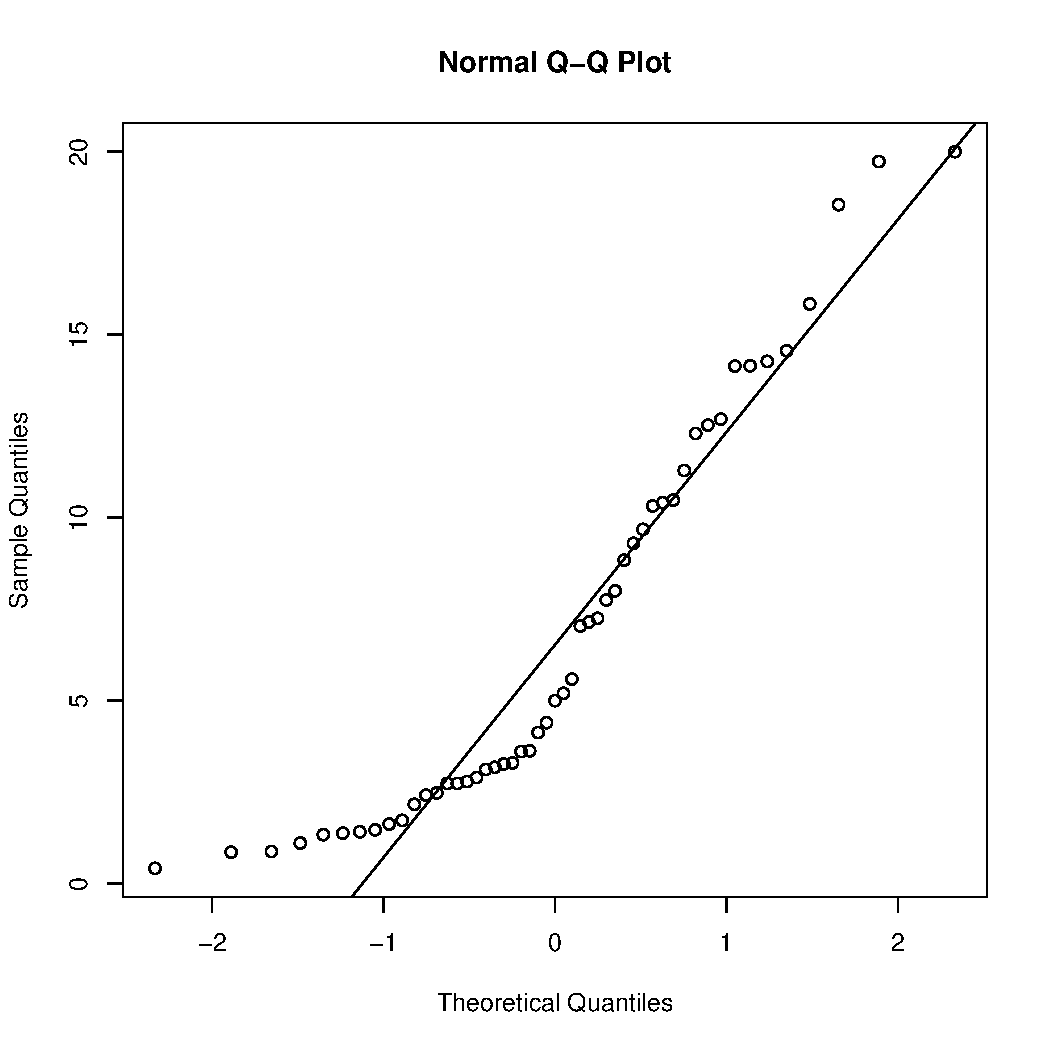
\includegraphics[width=.45\textwidth]{figure/unnamed-chunk-21} 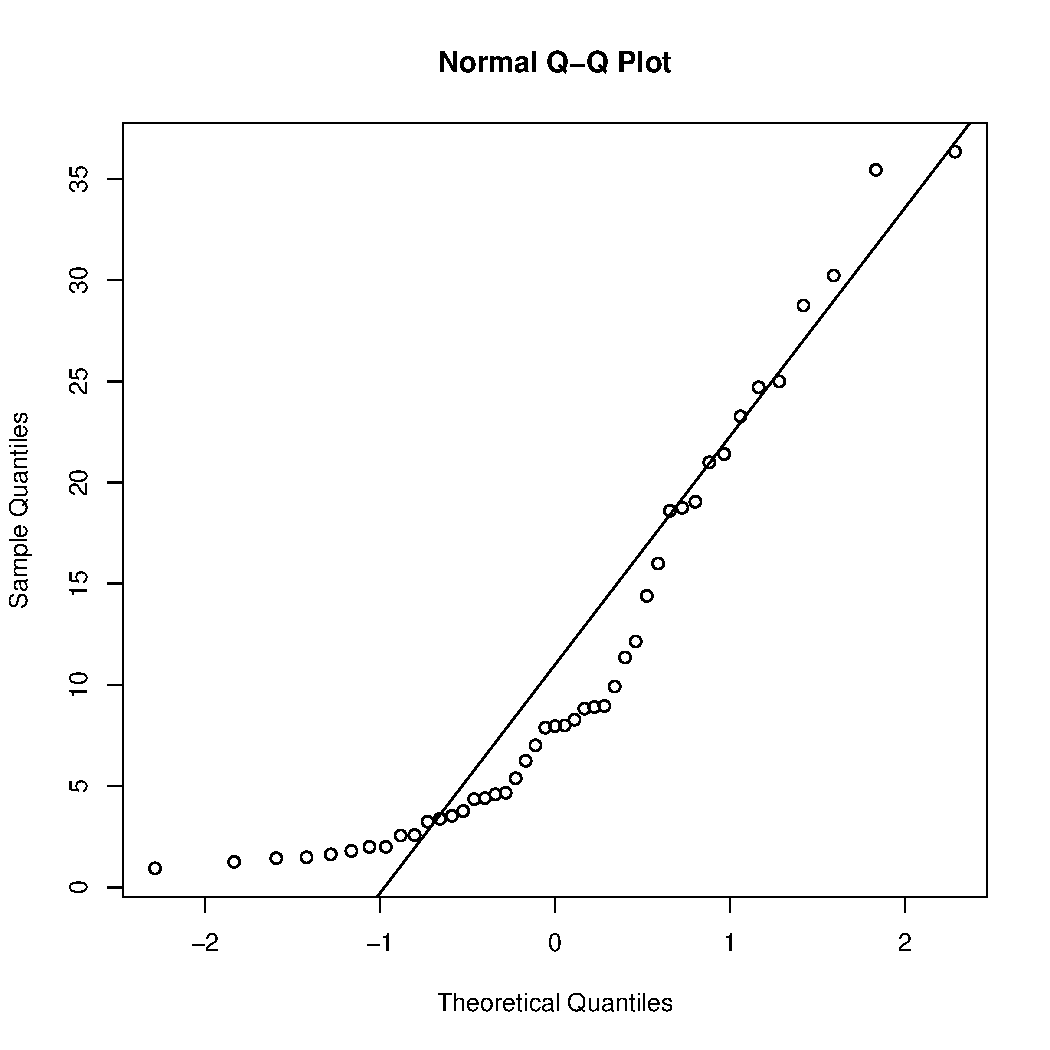
\includegraphics[width=.45\textwidth]{figure/unnamed-chunk-22} 

}


\end{knitrout}


\end{shaded}
\item[3.] What conclusions can you reach about the effect of the Litter size on Relative Brain weights?
\begin{shaded}
I don't see a straight line or functional relationship in the qqplot, so I don't think we can
make any conclusion.  Both distributions are right skewed, from the qqnorm plots.
\end{shaded}
\ee
\vvn\vvn
{\bf III.\ ( 15 Points )}\ \  A data value Y is an outlier if
\v\h $Y < Q(.25)-1.5*IQR \ \ \hbox{or} \ \ Y > Q(.75)+1.5*IQR$
\vvn
\h Calculate the probability that a randomly selected observation
is a outlier  if the
distribution of Y is
\begin{enumerate}
\item[1.] exponential
\begin{shaded}
Of course, this is using a single "standard" distribution for each case, when we
should leave the parameters in to see the functional dependency; this seemed like fun though.
\begin{knitrout}
\definecolor{shadecolor}{rgb}{0.969, 0.969, 0.969}\color{fgcolor}\begin{kframe}
\begin{alltt}
prob.of.outlier <- \hlfunctioncall{function}(dist) \{
    d <- \hlfunctioncall{paste}(\hlstring{"p"}, dist, sep = \hlstring{""})
    q <- \hlfunctioncall{paste}(\hlstring{"q"}, dist, sep = \hlstring{""})
    left <- \hlfunctioncall{eval}(\hlfunctioncall{call}(q, 0.25))
    right <- \hlfunctioncall{eval}(\hlfunctioncall{call}(q, 0.75))
    IQR <- right - left
    lower <- \hlfunctioncall{eval}(\hlfunctioncall{call}(d, left - 1.5 * IQR, lower.tail = TRUE))
    upper <- \hlfunctioncall{eval}(\hlfunctioncall{call}(d, right + 1.5 * IQR, lower.tail = FALSE))
    \hlfunctioncall{list}(left.endpoint = lower, right.endpoint = upper)
\}
\hlfunctioncall{prob.of.outlier}(\hlstring{"exp"})
\end{alltt}
\begin{verbatim}
## $left.endpoint
## [1] 0
## 
## $right.endpoint
## [1] 0.04811
\end{verbatim}
\end{kframe}
\end{knitrout}


\end{shaded}
\vfil
\newpage
\item[2.] Weibull

\begin{shaded}
Have to modify {\tt prob.of.outlier} since {\sl shape} parameter isn't given a default.
Let {\sl shape} be 1; i.e., an exponential, so that we should get answer above.
\begin{knitrout}
\definecolor{shadecolor}{rgb}{0.969, 0.969, 0.969}\color{fgcolor}\begin{kframe}
\begin{alltt}
W_prob.of.outlier_W <- \hlfunctioncall{function}(dist, shape.param = 1) \{
    d <- \hlfunctioncall{paste}(\hlstring{"p"}, dist, sep = \hlstring{""})
    q <- \hlfunctioncall{paste}(\hlstring{"q"}, dist, sep = \hlstring{""})
    left <- \hlfunctioncall{eval}(\hlfunctioncall{call}(q, 0.25, shape = shape.param))
    right <- \hlfunctioncall{eval}(\hlfunctioncall{call}(q, 0.75, shape = shape.param))
    IQR <- right - left
    lower <- \hlfunctioncall{eval}(\hlfunctioncall{call}(d, left - 1.5 * IQR, shape = shape.param, lower.tail = TRUE))
    upper <- \hlfunctioncall{eval}(\hlfunctioncall{call}(d, right + 1.5 * IQR, shape = shape.param, lower.tail = FALSE))
    \hlfunctioncall{list}(left.endpoint = lower, right.endpoint = upper)
\}
\hlfunctioncall{W_prob.of.outlier_W}(\hlstring{"weibull"})
\end{alltt}
\begin{verbatim}
## $left.endpoint
## [1] 0
## 
## $right.endpoint
## [1] 0.04811
\end{verbatim}
\end{kframe}
\end{knitrout}

Of course, any shape parameter can be substituted:
\begin{knitrout}
\definecolor{shadecolor}{rgb}{0.969, 0.969, 0.969}\color{fgcolor}\begin{kframe}
\begin{alltt}
\hlfunctioncall{W_prob.of.outlier_W}(\hlstring{"weibull"}, 1:5)
\end{alltt}
\begin{verbatim}
## $left.endpoint
## [1] 0.000000 0.000000 0.000000 0.001706 0.005043
## 
## $right.endpoint
## [1] 0.0481125 0.0103037 0.0030085 0.0011264 0.0005086
\end{verbatim}
\end{kframe}
\end{knitrout}

\end{shaded}
\item[3.] uniform on (0,1)
\begin{shaded}
\begin{knitrout}
\definecolor{shadecolor}{rgb}{0.969, 0.969, 0.969}\color{fgcolor}\begin{kframe}
\begin{alltt}
\hlfunctioncall{prob.of.outlier}(\hlstring{"unif"})
\end{alltt}
\begin{verbatim}
## $left.endpoint
## [1] 0
## 
## $right.endpoint
## [1] 0
\end{verbatim}
\end{kframe}
\end{knitrout}

\end{shaded}
\item[4.] normal
\begin{shaded}
\begin{knitrout}
\definecolor{shadecolor}{rgb}{0.969, 0.969, 0.969}\color{fgcolor}\begin{kframe}
\begin{alltt}
\hlfunctioncall{prob.of.outlier}(\hlstring{"norm"})
\end{alltt}
\begin{verbatim}
## $left.endpoint
## [1] 0.003488
## 
## $right.endpoint
## [1] 0.003488
\end{verbatim}
\end{kframe}
\end{knitrout}

\end{shaded}
\item[5.] t with df=2
\begin{shaded}
\begin{knitrout}
\definecolor{shadecolor}{rgb}{0.969, 0.969, 0.969}\color{fgcolor}\begin{kframe}
\begin{alltt}
T_prob.of.outlier_T <- \hlfunctioncall{function}(dist, df.param) \{
    d <- \hlfunctioncall{paste}(\hlstring{"p"}, dist, sep = \hlstring{""})
    q <- \hlfunctioncall{paste}(\hlstring{"q"}, dist, sep = \hlstring{""})
    left <- \hlfunctioncall{eval}(\hlfunctioncall{call}(q, 0.25, df = df.param))
    right <- \hlfunctioncall{eval}(\hlfunctioncall{call}(q, 0.75, df = df.param))
    IQR <- right - left
    lower <- \hlfunctioncall{eval}(\hlfunctioncall{call}(d, left - 1.5 * IQR, df = df.param, lower.tail = TRUE))
    upper <- \hlfunctioncall{eval}(\hlfunctioncall{call}(d, right + 1.5 * IQR, df = df.param, lower.tail = FALSE))
    \hlfunctioncall{list}(left.endpoint = lower, right.endpoint = upper)
\}
\hlfunctioncall{T_prob.of.outlier_T}(\hlstring{"t"}, 2:5)
\end{alltt}
\begin{verbatim}
## $left.endpoint
## [1] 0.04117 0.02751 0.02072 0.01676
## 
## $right.endpoint
## [1] 0.04117 0.02751 0.02072 0.01676
\end{verbatim}
\end{kframe}
\end{knitrout}


\end{shaded}
\end{enumerate}
\vnn\vnn
{\bf IV.\ ( 10 points) } \ \  Nylon bars were tested for brittleness. Each of 280
bars was molded under similar conditions and was tested by placing a specified
stress at 5 locations on the bar. Assuming
that each bar has uniform composition, the number of breaks on a given bar
should be binomially distributed with an unknown probability p of breaking.
The following table summarizes the outcome of the experiment:
\begin{center}
\begin{tabular}{|c|cccccc|c|} \hline
Breaks/Bar &  0   &   1 &  2 & 3 & 4 & 5 & total \\
Frequency  &  121 & 110 & 38 & 7 & 3 & 1 & 280   \\ \hline
\end{tabular}
\end{center}
\begin{enumerate}
\item[] Use a GOF test to evaluate whether the data appears to be from
a binomial model.
\end{enumerate}
\begin{shaded}
We need an estimate of $\theta$:
\begin{knitrout}
\definecolor{shadecolor}{rgb}{0.969, 0.969, 0.969}\color{fgcolor}\begin{kframe}
\begin{alltt}
(theta.hat <- \hlfunctioncall{as.numeric}(\hlfunctioncall{crossprod}(\hlfunctioncall{c}(0, 1, 2, 3, 4, 5), \hlfunctioncall{c}(121, 110, 38, 7, 3, 1))/(280 * 5)))
\end{alltt}
\begin{verbatim}
## [1] 0.16
\end{verbatim}
\end{kframe}
\end{knitrout}

Now calculate $\hat{p}_i$, $E$ and the ratio:
\begin{knitrout}
\definecolor{shadecolor}{rgb}{0.969, 0.969, 0.969}\color{fgcolor}\begin{kframe}
\begin{alltt}
(p.hat <- \hlfunctioncall{dbinom}(0:5, size = 5, prob = theta.hat))
\end{alltt}
\begin{verbatim}
## [1] 0.4182119 0.3982971 0.1517322 0.0289014 0.0027525 0.0001049
\end{verbatim}
\begin{alltt}
(E <- 280 * p.hat)
\end{alltt}
\begin{verbatim}
## [1] 117.09934 111.52318  42.48502   8.09239   0.77070   0.02936
\end{verbatim}
\begin{alltt}
O <- \hlfunctioncall{c}(121, 110, 38, 7, 3, 1)
(ratio <- \hlfunctioncall{sum}((O - E)^2/E))
\end{alltt}
\begin{verbatim}
## [1] 39.31
\end{verbatim}
\begin{alltt}
df <- 6 - 1 - 1
(p.val <- 1 - \hlfunctioncall{pchisq}(ratio, df))
\end{alltt}
\begin{verbatim}
## [1] 6.014e-08
\end{verbatim}
\end{kframe}
\end{knitrout}

This is a poor fit.
\end{shaded}
\vvn\vvn
{\bf V.\ ( 16 points)}  \ \  A major problem in the Gulf of Mexico is the excessive capture of game fish by shrimpers.
A random sample of the catch of 50 shrimpers yield the following data concerning the catch per unit effort (CPUE) of Red Snappers, a highly sought game fish. Let  $C_i$ be the CPUE for the ith shrimper. The data, $C_1, C_2,\ldots,C_{50}$ is given next.
\vvn
\begin{center}
\begin{tabular}{|cccccccccc|}\hline
0.6 &  0.7 & 1.1  &  1.3 & 1.8  &  2.0 &  2.3 &  2.7 &  2.9 &  3.1\\
3.9 & 4.3  & 4.4  & 4.9  &  5.2 &  5.4 & 6.1  &  6.8 &  7.1 &  8.0\\
9.4 &10.3  & 12.9 & 15.9 &  16.0& 22.0 & 22.2 &22.5  &  23.0& 23.1\\
23.9&26.5  & 26.7 & 28.4 & 28.5 & 32.2 &  40.2&42.5  &  47.2& 48.3\\
55.8&57.0& 57.2 & 64.9 &  67.6& 71.3 & 79.5 & 114.5& 128.6&293.5 \\
  \hline
\end{tabular}
\end{center}
\vvn
\be
\item[1.] CPUE data is often modelled using a Log-Normal distribution. Does the above data appear to be from a Log-Normal distribution? Explain your answer with both
a normal reference distribution plot and a GOF test.
\begin{shaded}
\begin{knitrout}
\definecolor{shadecolor}{rgb}{0.969, 0.969, 0.969}\color{fgcolor}\begin{kframe}
\begin{alltt}
CPUE <- \hlfunctioncall{c}(0.6, 0.7, 1.1, 1.3, 1.8, 2, 2.3, 2.7, 2.9, 3.1, 3.9, 4.3, 4.4, 4.9, 5.2, 5.4, 6.1, 
    6.8, 7.1, 8, 9.4, 10.3, 12.9, 15.9, 16, 22, 22.2, 22.5, 23, 23.1, 23.9, 26.5, 26.7, 28.4, 
    28.5, 32.2, 40.2, 42.5, 47.2, 48.3, 55.8, 57, 57.2, 64.9, 67.6, 71.3, 79.5, 114.5, 128.6, 
    293.5)
\hlfunctioncall{qqnorm}(\hlfunctioncall{log}(CPUE))
\hlfunctioncall{qqline}(\hlfunctioncall{log}(CPUE))
\end{alltt}
\end{kframe}

{\centering 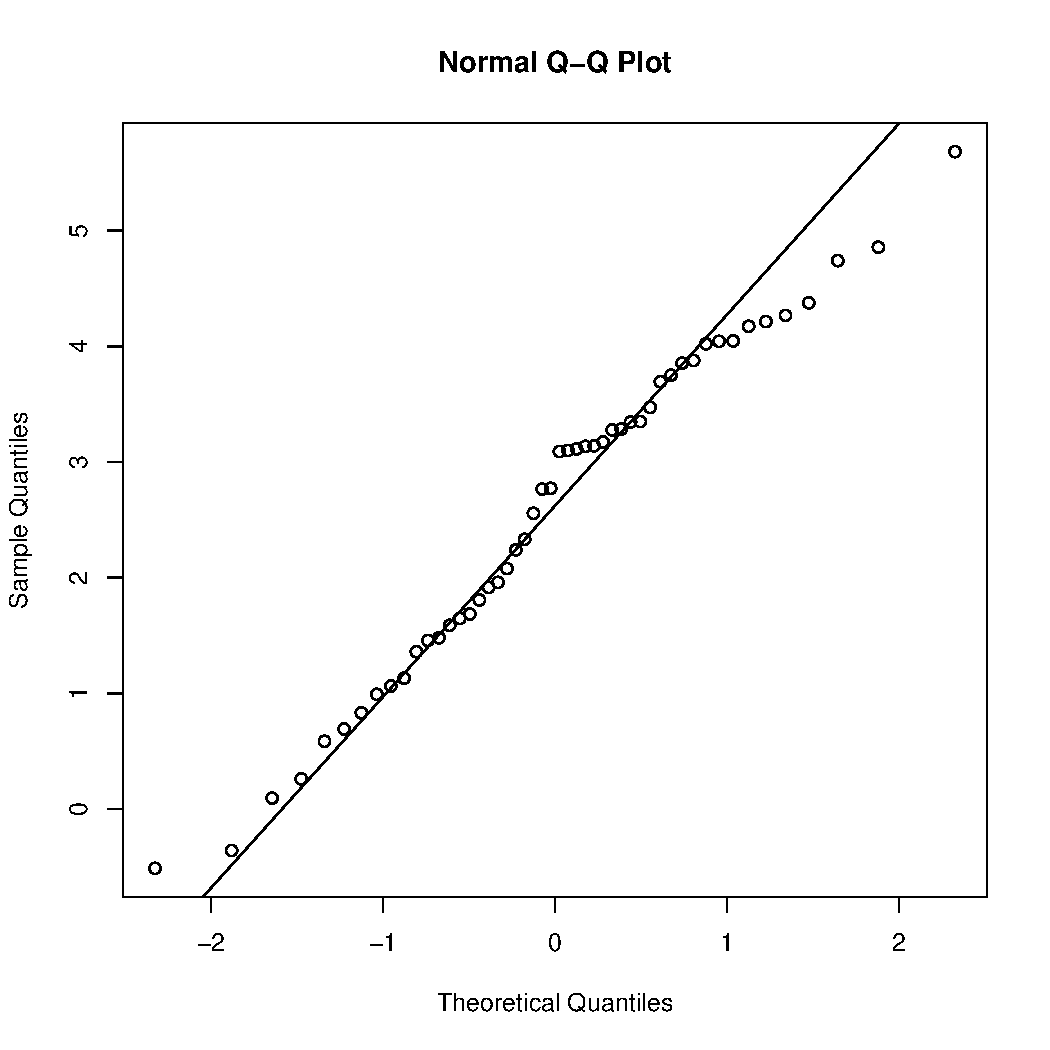
\includegraphics[width=.6\textwidth]{figure/unnamed-chunk-111} 

}

\begin{kframe}\begin{alltt}
\hlfunctioncall{library}(fitdistrplus)
\hlfunctioncall{descdist}(\hlfunctioncall{log}(CPUE), boot = 1000)
\end{alltt}
\begin{verbatim}
## summary statistics
## ------
## min:  -0.5108   max:  5.682 
## median:  2.932 
## mean:  2.591 
## estimated sd:  1.453 
## estimated skewness:  -0.236 
## estimated kurtosis:  2.362
\end{verbatim}
\end{kframe}

{\centering 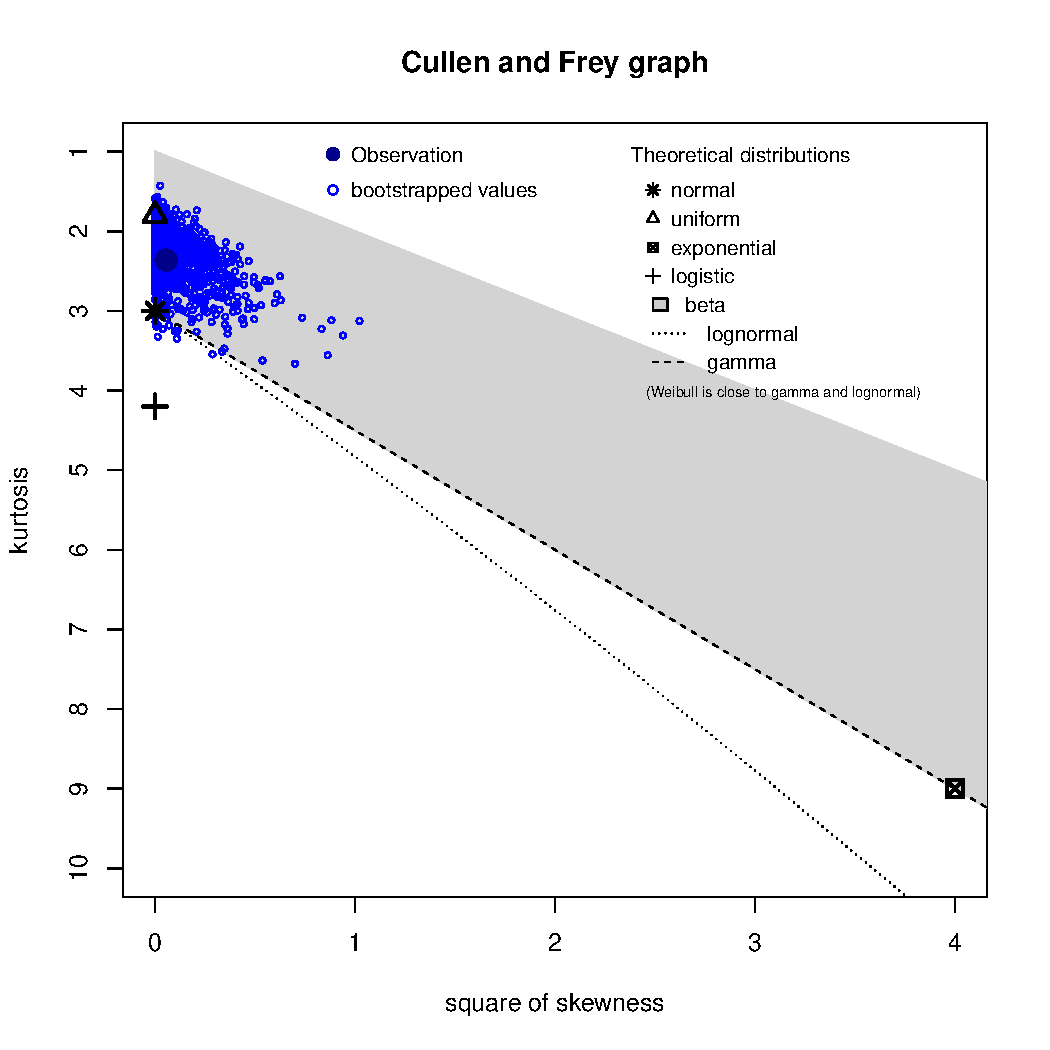
\includegraphics[width=.6\textwidth]{figure/unnamed-chunk-112} 

}

\begin{kframe}\begin{alltt}
f <- \hlfunctioncall{fitdist}(CPUE, \hlstring{"lnorm"})
\hlfunctioncall{plot}(f)
\end{alltt}
\end{kframe}

{\centering 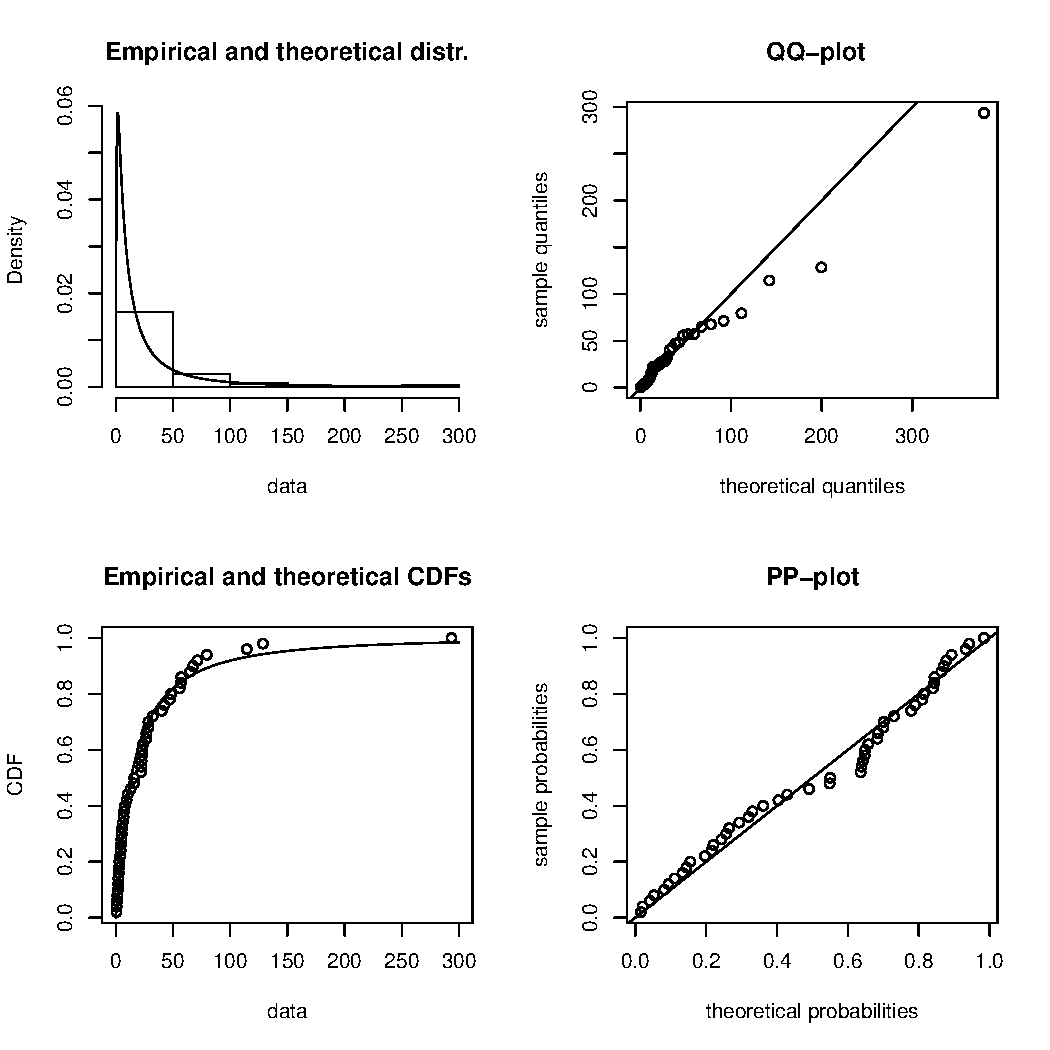
\includegraphics[width=.6\textwidth]{figure/unnamed-chunk-113} 

}

\begin{kframe}\begin{alltt}
\hlfunctioncall{gofstat}(f, print.test = TRUE)
\end{alltt}
\begin{verbatim}
## Kolmogorov-Smirnov statistic:  0.136 
## Kolmogorov-Smirnov test:  not rejected 
##    The result of this test may be too conservative as it  
##    assumes that the distribution parameters are known
## Cramer-von Mises statistic:  0.09077 
## Cramer-von Mises test:  not rejected 
## Anderson-Darling statistic:  0.4774 
## Anderson-Darling test:  not rejected
\end{verbatim}
\end{kframe}
\end{knitrout}

Used a bit of a black box here, but betweenthe Cullen-Fry graph of the logged data 
and the GOF tests, it seems the fit is pretty good.  There is one large value that
may be causing undue influence.
\end{shaded}
\item[2.] Use the Box-Cox transformation of the CPUE data to
  determine the most appropriate power transformation to transform
  the CPUE distribution to Normality. How does the fit from the Box-Cox transformation compare to the fit for the log transformation?
\begin{shaded}
\begin{knitrout}
\definecolor{shadecolor}{rgb}{0.969, 0.969, 0.969}\color{fgcolor}\begin{kframe}
\begin{alltt}
bc <- \hlfunctioncall{function}(y, theta) \{
    \hlfunctioncall{if} (theta == 0) 
        \hlfunctioncall{return}(\hlfunctioncall{log}(y)) else \hlfunctioncall{return}((y^theta - 1)/theta)
\}
theta <- \hlfunctioncall{seq}(0, 3, by = 0.25)
orig.mat <- \hlfunctioncall{matrix}(\hlfunctioncall{rep}(CPUE, \hlfunctioncall{length}(theta)), nrow = \hlfunctioncall{length}(theta), byrow = TRUE)
trans.mat <- \hlfunctioncall{apply}(orig.mat, 1, bc, theta)
\end{alltt}


{\ttfamily\noindent\textcolor{warningcolor}{\#\# Warning: the condition has length > 1 and only the first element will be used}}

{\ttfamily\noindent\textcolor{warningcolor}{\#\# Warning: the condition has length > 1 and only the first element will be used}}

{\ttfamily\noindent\textcolor{warningcolor}{\#\# Warning: the condition has length > 1 and only the first element will be used}}

{\ttfamily\noindent\textcolor{warningcolor}{\#\# Warning: the condition has length > 1 and only the first element will be used}}

{\ttfamily\noindent\textcolor{warningcolor}{\#\# Warning: the condition has length > 1 and only the first element will be used}}

{\ttfamily\noindent\textcolor{warningcolor}{\#\# Warning: the condition has length > 1 and only the first element will be used}}

{\ttfamily\noindent\textcolor{warningcolor}{\#\# Warning: the condition has length > 1 and only the first element will be used}}

{\ttfamily\noindent\textcolor{warningcolor}{\#\# Warning: the condition has length > 1 and only the first element will be used}}

{\ttfamily\noindent\textcolor{warningcolor}{\#\# Warning: the condition has length > 1 and only the first element will be used}}

{\ttfamily\noindent\textcolor{warningcolor}{\#\# Warning: the condition has length > 1 and only the first element will be used}}

{\ttfamily\noindent\textcolor{warningcolor}{\#\# Warning: the condition has length > 1 and only the first element will be used}}

{\ttfamily\noindent\textcolor{warningcolor}{\#\# Warning: the condition has length > 1 and only the first element will be used}}

{\ttfamily\noindent\textcolor{warningcolor}{\#\# Warning: the condition has length > 1 and only the first element will be used}}\end{kframe}
\end{knitrout}

\end{shaded}
\ee
\vfill\newpage
\vvn\vvn
{\bf VI.\ ( 20 Points )}\ \  A random sample of 500 data values are selected from
four separate processes having cdf's, $F_1, F_2, F_3, F_4$. The plot of the
sample quantile versus a standard normal quantile for each of the four samples
is given below. For each of these plots,
{\bf SELECT ONE} of the following
distributions to
describe the pdf which generated the data. Hint: make sure to take into consideration
the size of values associated with each distribution.
\vskip4mm
\noindent
\small
\begin{enumerate}
\item[(A)] Cauchy($\theta_1=.35,\theta_2=1$) \hskip2.52in  {\bf \large Plot 1
  \underbar { \  \  \  \  \  \  \ \  \  \  \  \  \  \ }}
\item[(B)] t with df=35
\item[(C)] Logistic($\theta_1=.35,\theta_2=1$)\hskip2.54in  {\bf \large Plot 2
  \underbar { \  \  \  \  \  \  \ \  \  \  \  \  \  \ }}
\item[(D)] Beta($\alpha=2,\beta=6$)
\item[(E)] Uniform(0,.7)\hskip3.14in{\bf \large Plot 3 \underbar { \  \  \
    \  \  \  \ \  \  \  \  \  \  \ }}
\item[(F)] Normal($\mu=.35,\sigma=1$)
\item[(G)] Exponential($\beta=80$)\hskip2.76in{\bf \large Plot 4 \underbar { \  \
    \  \  \  \  \ \  \  \  \  \  \  \ }}
\item[(H)] Weibull($\gamma=0.7,\beta=20$)
\item[(I)] Gamma($\alpha=1.2,\beta=25$)
\item[(J)] Mixture of 90\% Normal($10,1$) \& 10\% Normal($30,(3)^2$)
\item[(K)] Mixture of 10\% Normal($10,1$) \& 90\% Normal($30,(1)^2$)
\item[(L)] Normal($\mu=20,\sigma=1$)
\end{enumerate}
\vskip4mm
% \begin{center}
% \noindent
% \rotatebox{270}{
% \psfig{file=u:/exams/stat641/e1f06_4p.ps,height=5in,width=5in}}
% \end{center}
\vvn\vvn

\vfill\newpage
\vskip5mm
\vvn
{\bf VII. \ \ (18 points)}\ \ {\bf Multiple Choice Questions}
Select the letter of the {\bf BEST} answer. Justify your answer in 20 words or less.
\vskip2mm
\noindent
\be
\item[1.]   The Anderson-Darling (AD) GOF statistic
  is prefered to the Kolmogorov-Smirnov (KS) GOF statistic for
testing the goodness-of-fit of a continuous pdf because
\be
\item[A.] AD is a more modern procedure.
\item[B.] AD has a more accurate p-value than does KS.
\item[C.] AD is less likely to falsely declare that a distribution does not fit the collected data.
\item[D.] AD is more likely to declare that a distribution function does not fit the edf, especially in
the tails of the distribution.
\item[E.] All of the above are true.
\ee
\item[2.]  An entomologist is recording $Y$, the saturation deficit (a function of temperature and relative humidity) of Lone Star ticks. In order to
be very precise in his study of these ticks, the entomologist wants to determine if the cdf of $Y$, $F(y)$ has
a particular form $F_o(y)$. The entomologist measures the value of $Y$ for each of 213 randomly selected Lone Star ticks.
Which of the following procedures is best for determining whether $F=F_o$?
\be
\item[A.]  Anderson-Darling statistic.
\item[B.]  Kolmogorov-Smirnov statistic.
\item[C.]  Chi-square Goodness-of-Fit statistic.
\item[D.]  Shapiro-Wilks statistic.
\item[E.] depends on the shape of $F_o$.
\ee
\item[3.]  The Anderson-Darling GOF statistic is
referred to as a distribution-free statistic when the continuous cdf $F_o$ is completely specified because
\be
\item[A.] the distribution of the  statistic depends only on location-scale parameters.
\item[B.] the distribution of the statistic has a $N(0,1)$ distribution for large $n$.
\item[C.] the distribution of the statistic does not depend on location-scale parameters.
\item[D.] the distribution of the statistic is the same for choices of $F_o$, provided it is continuous.
\item[E.] none of the above are valid reasons
\ee
\item[4.] The Anderson-Darling statistic is preferred
to the Chi-square statistic in testing $H_o:F=F_o$ based on a random
sample $X_1, \cdots, X_n$ from a continuous cdf $F$ because
\be
\item[A.] the Anderson-Darling is more likely to maintain its level of Type I error.
\item[B.] the number of degrees of freedom for the Anderson-Darling are larger than those for the Chi-squared test.
\item[C.] the probability of Type I error is higher for the Chi-squared test than for the Anderson-Darling.
\item[D.] the Anderson-Darling test is more likely to correctly detect that $F$ is not equal to $F_o$.
\item[E.] none of the above
\ee
\item[5.)] An plant physiologist is studying the infestation rate of potato bud insects on genetically altered potato plants.
The researcher measures the number, $Y_1,\cdots,Y_{300}$, of  potato bud insects on 300 randomly selected genetically altered plants. In order to
model the factors affecting the infestation rate, the researcher wants to determine which of five possible cdfs, $F_1, \cdots, F_5$ best fits  the cdf of $Y$, $F(y)$. Which of the following tests would be the most appropriate procedure  for determining which of the five cdfs is the best fit?
\be
\item[A.] Anderson-Darling statistic
\item[B.] Kolmogorov-Smirnov statistic
\item[C.] Chi-square Goodness-of-Fit statistic
\item[D.] Shapiro-Wilks statistic
\item[E.] none of the above would be appropriate, they all deal with a single cdf
\ee
\item[6.] An estimator $\hat\theta_{max}$ of the maximum stress load of a new alloy has been developed.
A statistician conjectures that the sampling distribution of  $\hat\theta_{max}$ is Weibull with parameters $(\beta=10,\gamma=.2)$. A large scale simulation study was conducted to evaluate this claim.
A simulation was run with 5000 replications of $n=10$ data values resulting in 5000 values of $\hat\theta_{max}$.
A Weibull reference distribution plot was constructed yielding the following plot:
\vn
%\psfig{file=u:/exams/stat641/fnf06_weib.ps,width=6in,height=4in}
%\psfig{file=c:/exams/stat641/fnf06_weib.ps,width=5in,height=3in}
\vn
The Anderson-Darling GOF of the Weibull $(\beta=10,\gamma=.2)$ model yielded a p-value of 0.001.
Why does the reference distribution plot and the Anderson-Darling statistic appear to be contradictory in their assessment of
the sampling distribution of $\hat\theta_{max}$?
\be
\item[A.] There is no contradiction.
\item[B.] The vertical scale on the reference distribution plot is deceptive.
\item[C.] The distribution must be incorrect.
\item[D.] With 5000 values of $\hat\theta_{max}$, the Anderson-Darling test is extremely sensitive to slight deviations
from the Weibull model.
\item[E.] The Anderson-Darling test is not a very powerful test for the Weibull distribution.
\ee
\ee
\vnn\vnn
\vfill
\end{document}
